\section{Experiments and Results}

\subsection{Dataset}

We evaluate on the ISIC 2019 Challenge dataset
\cite{combalia2019bcn20000,tschandl2018ham10000} containing 25,331
dermoscopic images across 8 populated diagnostic categories. The class
distribution exhibits significant imbalance: Nevus (NV) comprises 50.83\% of
samples while Dermatofibroma (DF) represents only 0.94\%. We employ stratified
splitting with 70\% training (17,731 images), 15\% validation (3,800
images), and 15\% test (3,800 images).

\begin{table}[t]
    \centering
    \caption{Class distribution in the ISIC 2019 dataset.}
    \label{tab:distribution}
    \begin{tabular}{lrr}
        \toprule
        Class                         & Count  & Percentage \\
        \midrule
        NV (Nevus)                    & 12,875 & 50.83\%    \\
        MEL (Melanoma)                & 4,522  & 17.85\%    \\
        BCC (Basal Cell Carcinoma)    & 3,323  & 13.12\%    \\
        BKL (Benign Keratosis)        & 2,624  & 10.36\%    \\
        AK (Actinic Keratosis)        & 867    & 3.42\%     \\
        SCC (Squamous Cell Carcinoma) & 628    & 2.48\%     \\
        VASC (Vascular)               & 253    & 1.00\%     \\
        DF (Dermatofibroma)           & 239    & 0.94\%     \\
        \bottomrule
    \end{tabular}
\end{table}

\subsection{Classification Performance}

Table \ref{tab:results} reports overall test-set performance. Because half the
test set is a single class, we treat the imbalance-aware measures as the primary
result: the model reaches 81.67\% balanced accuracy (the mean per-class recall)
and a macro-averaged F1 of 0.804, alongside 85.61\% overall accuracy and a
weighted F1 of 0.856. The gap between the weighted and macro figures is the
expected consequence of the class imbalance rather than a separate finding.

\begin{table}[t]
    \centering
    \caption{Overall test set performance metrics. Macro and balanced measures
        weight every class equally and are the primary numbers given the class
        imbalance.}
    \label{tab:results}
    \begin{tabular}{lc}
        \toprule
        Metric               & Value  \\
        \midrule
        Balanced accuracy    & 0.8167 \\
        F1 score (macro)     & 0.8036 \\
        ROC-AUC (macro, OvR) & [TODO] \\
        \midrule
        Accuracy             & 0.8561 \\
        Precision (weighted) & 0.8600 \\
        Recall (weighted)    & 0.8561 \\
        F1 score (weighted)  & 0.8564 \\
        \bottomrule
    \end{tabular}
    % Balanced accuracy = macro recall (Table 3). ROC-AUC produced by
    % `melanoma eval`; fill in after regenerating with saved probabilities.
\end{table}

Table \ref{tab:perclass} provides the per-class breakdown, including the
one-vs-rest specificity that complements recall (sensitivity) for a clinical
reading. The model performs best on Nevus (F1=0.91) and BCC (F1=0.89), which
benefit from larger sample sizes. Melanoma detection reaches F1=0.77 with
80.57\% precision and 74.52\% recall (sensitivity). Minority classes are more
variable: DF reaches 86.11\% recall from only 36 test samples, whereas AK
recall is 63.85\%.

\begin{table}[t]
    \centering
    \caption{Per-class classification performance. Recall is the per-class
        sensitivity; specificity and ROC-AUC are computed one-vs-rest.}
    \label{tab:perclass}
    \begin{tabular}{lccccr}
        \toprule
        Class     & Precision & Recall & F1     & Spec.\ / AUC & Support \\
        \midrule
        MEL       & 0.8057    & 0.7452 & 0.7743 & [TODO]       & 679     \\
        NV        & 0.9255    & 0.9011 & 0.9131 & [TODO]       & 1931    \\
        BCC       & 0.8579    & 0.9319 & 0.8934 & [TODO]       & 499     \\
        AK        & 0.7545    & 0.6385 & 0.6917 & [TODO]       & 130     \\
        BKL       & 0.6900    & 0.8270 & 0.7523 & [TODO]       & 393     \\
        DF        & 0.6200    & 0.8611 & 0.7209 & [TODO]       & 36      \\
        VASC      & 0.8947    & 0.8947 & 0.8947 & [TODO]       & 38      \\
        SCC       & 0.8519    & 0.7340 & 0.7886 & [TODO]       & 94      \\
        \midrule
        Macro avg & 0.8000    & 0.8167 & 0.8036 & [TODO]       & 3800    \\
        \bottomrule
    \end{tabular}
    % Specificity and per-class AUC produced by `melanoma eval` from saved
    % probabilities; fill in after regenerating.
\end{table}

\subsection{Explainability Outputs}

% NOTE: the uncertainty values quoted in the two figures below and in the
% surrounding text were produced by the earlier MC-dropout implementation.
% After the switch to full-network MC dropout with a mutual-information
% epistemic term (Section on MC Dropout), regenerate these panels with
% `poe paper-figures` and update the quoted predictive/epistemic/aleatoric
% numbers accordingly.
Figures \ref{fig:sample_benign} and \ref{fig:sample_mel} show the full analysis
output for two test images with different risk profiles and reliability
assessments.

\begin{figure*}[t]
    \centering
    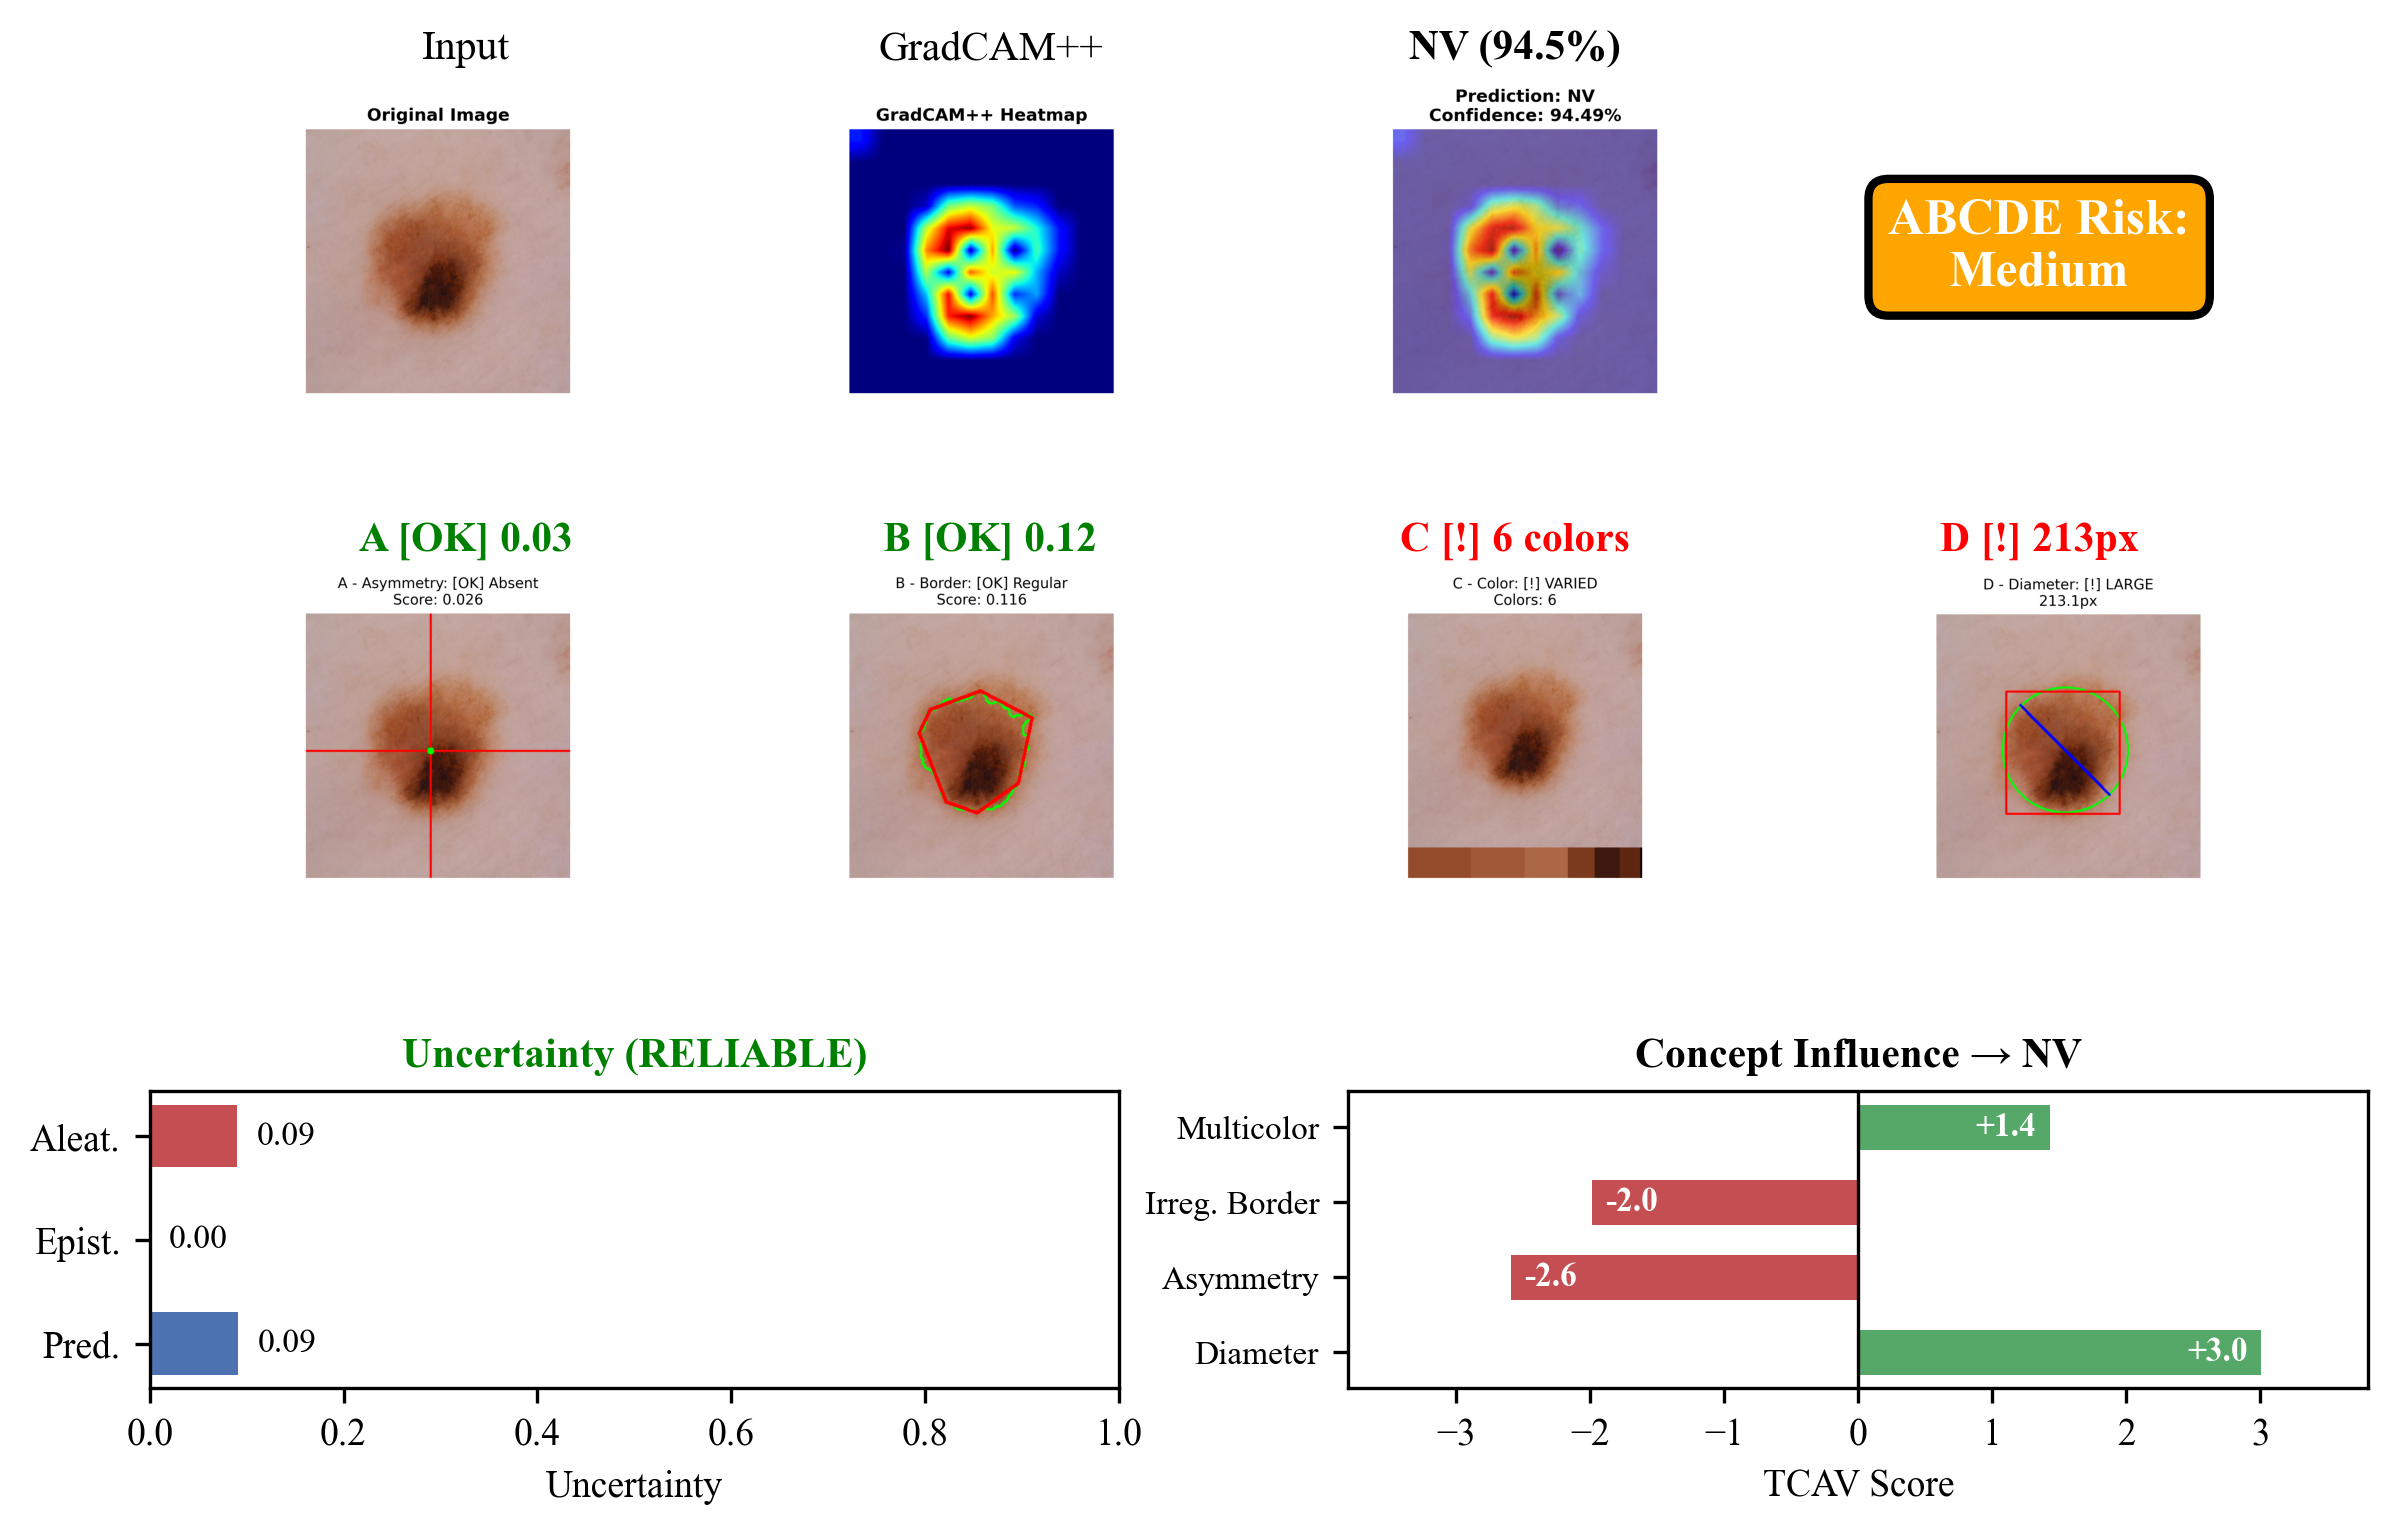
\includegraphics[width=0.95\textwidth]{figures/ISIC_0034335_paper.png}
    \caption{Analysis of a benign nevus (NV) with medium ABCDE risk. The model
        classifies with 94.49\% confidence. Top row: original image, GradCAM++
        heatmap, and overlay with prediction. Middle row: ABCDE criterion
        visualizations showing asymmetry axes, border contour, color palette, and
        diameter measurement. Bottom panels: uncertainty decomposition (left) and
        SGD-CAV concept importance scores (right).}
    \label{fig:sample_benign}
\end{figure*}

\begin{figure*}[t]
    \centering
    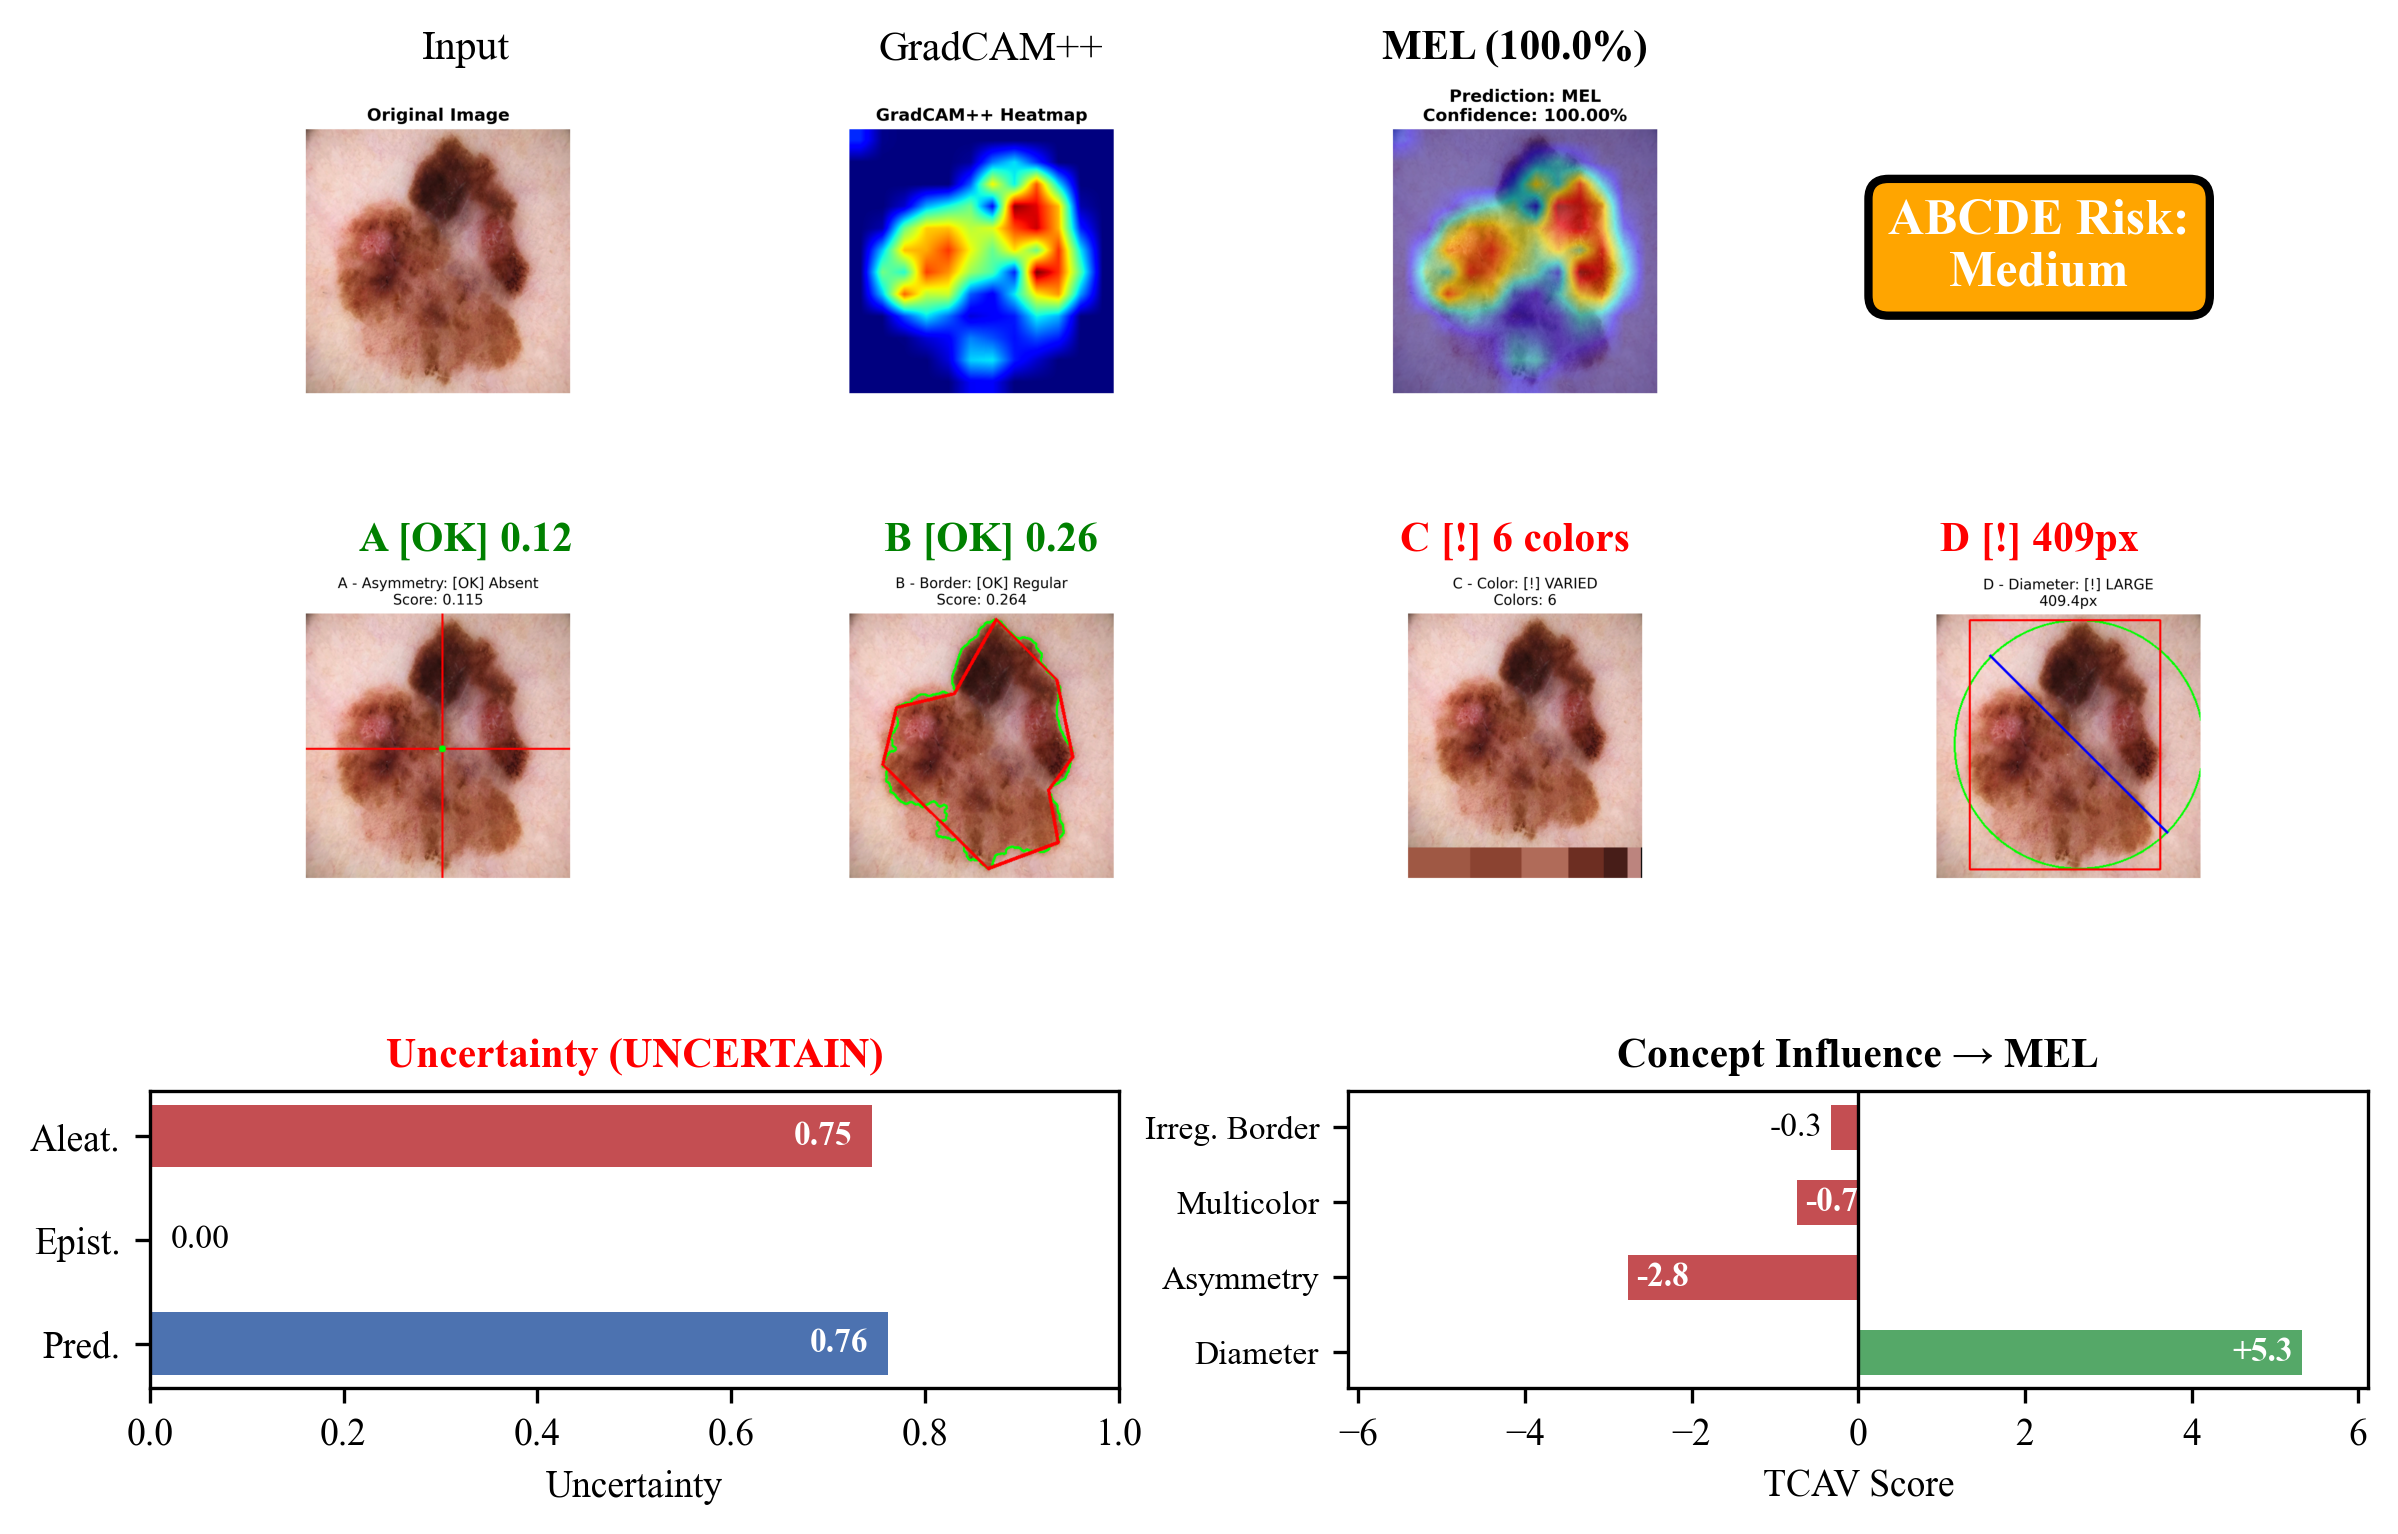
\includegraphics[width=0.95\textwidth]{figures/ISIC_0034376_paper.png}
    \caption{Analysis of a melanoma (MEL) with medium ABCDE risk. The model
        classifies with 100\% confidence but the uncertainty module flags this as
        ``UNCERTAIN'' due to high aleatoric uncertainty (0.75). ABCDE criteria show
        acceptable asymmetry (0.12) and borders (0.26), but flag multiple colors (6)
        and large diameter (409px). SGD-CAV analysis reveals large diameter strongly
        supports the prediction (+5.32) while asymmetry opposes it (-2.77).}
    \label{fig:sample_mel}
\end{figure*}

Figure \ref{fig:sample_benign} shows a correctly classified nevus with
94.49\% confidence. The GradCAM++ heatmap confirms the model focuses on the
lesion center. ABCDE analysis shows low asymmetry (0.026), regular borders
(0.116), but multiple colors (6) and larger diameter (213 pixels), yielding
medium risk. Uncertainty analysis reports low predictive uncertainty (0.088),
flagged as ``RELIABLE.'' SGD-CAV scores show large diameter (+2.29) and
multicolor (+0.53) supporting the prediction while asymmetry (-1.43) and
irregular border (-1.31) oppose it.

Figure \ref{fig:sample_mel} presents a melanoma classified with 100\%
confidence. Despite high confidence, the uncertainty module flags this as
``UNCERTAIN'' due to high predictive uncertainty (0.76) dominated by
aleatoric uncertainty (0.75), demonstrating that confidence and uncertainty
provide complementary information. ABCDE analysis shows acceptable asymmetry
(0.12) and regular borders (0.26), but flags multiple colors (6) and large
diameter (409 pixels). SGD-CAV concept scores show large diameter strongly
supports the melanoma prediction (+5.32) while asymmetry (-2.77), multicolor
(-0.74), and irregular border (-0.33) oppose it.

\subsection{Attention Alignment and Faithfulness}

We assess the attention maps in two ways. The alignment metrics ask whether
attention lands on clinically relevant regions: across the test set the mean
lesion attention is 0.60 and the mean border alignment is 0.53, both above the score
obtained by a random-attention map of the same resolution, indicating that the
model attends preferentially to the lesion and, more weakly, to its border
rather than the background.

Alignment alone does not establish that the highlighted regions are the ones the
model uses. We therefore also measure faithfulness with deletion and insertion
tests: pixels are removed from (or added to) the image in order of attention, and
we record how quickly the predicted probability falls (or rises). Summarised as
the area over the probability curve, GradCAM++ yields a deletion score of
\textbf{[TODO]} and an insertion score of \textbf{[TODO]}, compared with
\textbf{[TODO]} and \textbf{[TODO]} for random attention.%
% Numbers produced by `melanoma faithfulness`; fill in after the run.
The gap over the random control is the evidence that the maps reflect the
model's computation rather than incidental structure in the image.

\subsection{Reproducibility}
\label{sec:reproducibility}

All experiments use a fixed random seed and the training configuration described
in Section~\ref{sec:methods-training}. The reported test metrics are produced by
the released evaluation script, which also writes the per-sample predictions and
probabilities used for the ROC and faithfulness analyses. Reported confidence
intervals come from repeating training and evaluation across several seeds and
aggregating the resulting metrics. Code, configuration, and trained weights are
released to allow the numbers here to be regenerated.
